\chapter{Implementación}
\label{capitulo6}
\lhead{Capítulo 6. \emph{Dataset local}}


\section{Introducción}
El objetivo de este capítulo es explicar ka elaboración de un dataset visual inercial, a través de la construcción de un robot prototipo.
\clearpage



\section{Descripción general}\label{seccion-corte}

La estimación de odometría por medio de la fusión visual inercial fue desarrollada utilizando C++ como lenguaje de programación y ROS para la aplicación de los filtros inerciales y la visualización del movimiento del robot. Este programa utiliza un sólo hilo de ejecución, de forma que la odometría se estima de forma secuencial, pasando primero por estimar la orientación del robot utilizando el filtro inercial, y luego a estimar la traslación a partir de los residuales inerciales y la cámara. El formato de entrada de las imágenes y de los datos de la IMU fueron tomados de acuerdo al formato empleado en el EUROC Mav dataset.

En cuanto al dataset local realizado, también fue implementado utilizando C++ como lenguaje de programación, y utilizando una raspberry pi 3 para la adquisición de los datos de la imu y de la cámara, y utilizando 4 hilos de ejecución.


\section{Estimación de los residuales rotacionales}

Con el empleo de la IMU es posible obtener los cambios de orientación de la cámara y de su aceleración, siempre y cuando se encuentren sincronizadas las mediciones. Bajo esta restricción se tiene el residual de orientación de la IMU (${R}_{RES/IMU}$) , el cual representa el cambio de orientación de la IMU entre el frame actual y el anterior, tal como se presenta en la ecuación \ref{eq:residualIMU}.


\begin{equation}
{ R }_{ IMU2 }\quad =\quad { R }_{ IMU1 }*{ R }_{ RES/IMU }\quad \rightarrow \quad { R }_{ RES/IMU }\quad =\quad { { { R }_{ IMU1 } }^{ T }*\quad R }_{ IMU2 }
\label{eq:residualIMU} 
\end{equation}

De forma análoga, el residual de la cámara viene dado por:

\begin{equation}
{ R }_{ RES/CAM }\quad =\quad \quad { { R }_{ CAM1 } }^{ T }\quad .\quad { R }_{ CAM2 }
\label{eq:residualCAM} 
\end{equation}

Utilizando la ecuación \ref{eq:rotacionIMUCAM} en \ref{eq:residualCAM}, y las propiedades de la transpuesta del producto de matrices se tiene:

\begin{align}
{ R }_{ RES/CAM }\quad =\quad { { R }_{ CAM1 } }^{ T }.{ R }_{ CAM2 }\quad =\quad ({ R }_{ IMU1 }.{ R }_{ IMU-CAM })\quad ^{ T }.{ R }_{ IMU2 }.{ R }_{ IMU-CAM }\\ \quad \quad \quad \quad \quad \quad \quad \quad \quad =\quad ({ { R }_{ IMU-CAM } }^{ T }.{ { R }_{ IMU1 } }^{ T\quad  })\quad { R }_{ IMU2 }.{ R }_{ IMU-CAM }\\ \qquad \qquad \qquad ={ { \quad R }_{ IMU-CAM } }^{ T }.({ { R }_{ IMU1 } }^{ T\quad  }.{ R }_{ IMU2 }).{ R }_{ IMU-CAM }\\ \qquad \qquad \qquad =\quad { { R }_{ IMU-CAM } }^{ T }.({ { R }_{ IMU1 } }^{ T\quad  }.{ R }_{ IMU2 }).{ R }_{ IMU-CAM }
\label{eq:residualCAMProcedimiento} 
\end{align}

Y finalmente se obtiene:

\begin{equation}
{ R }_{ RES/CAM }\quad =\quad { { \quad R }_{ IMU-CAM } }^{ T }. { R }_{ RES/IMU } . { R }_{ IMU-CAM\\  }
\label{eq:residualCAMDeIMU} 
\end{equation}

De esta forma, utilizando la ecuación \ref{eq:residualCAMDeIMU}, es posible obtener el residual de orientación de la cámara directamente del residual de orientación de la imu.


\section{Estimación de los residuales traslacionales}


En general, en base a las transformaciones de cuerpo rígido se tiene:

\begin{equation}
\left[ \begin{matrix} { X }_{ 1 } \\ { Y }_{ 1 } \\ { Z }_{ 1 } \end{matrix} \right] \quad =\quad { R }_{ 1 }^{ 2 }.\left[ \begin{matrix} { X }_{ 2 } \\ { Y }_{ 2 } \\ { Z }_{ 2 } \end{matrix} \right] +{ P }_{ 1 }^{ 2 } 
\label{eq:TransformacionCAM1CAM2} 
\end{equation}


Donde $(X1, Y1, Z1)$ y $(X2, Y2, Z2)$ representan la ubicación en el espacio del punto característico detectado en la primera y segunda imagen, respectivamente, referidos a cada uno de los sistemas de referencia de la cámara cuando fue tomada la imagen. Utilizando la ecuación \ref{eq:ReproyeccionCAM} se obtiene:


\begin{equation}
{ Z }_{ 1 }\left[ \begin{matrix} \frac { u_{ 1 }-{ c }_{ x } }{ { f }_{ x } }  \\ \frac { { v }_{ 1 }-{ c }_{ y } }{ { f }_{ y } }  \\ 1 \end{matrix} \right] =\quad { R }_{ 1 }^{ 2 }.{ Z }_{ 2 }\left[ \begin{matrix} \frac { u_{ 2 }-{ c }_{ x } }{ { f }_{ x } }  \\ \frac { { v }_{ 2 }-{ c }_{ y } }{ { f }_{ y } }  \\ 1 \end{matrix} \right] +{ P }_{ 1 }^{ 2 }
\label{eq:TransformacionCAM1CAM2Reproyeccion} 
\end{equation}

Debemos recordar que a los puntos de la forma $s (X, Y, Z)$, donde $s$ es un factor de escala, le corresponden el mismo pixel de $(u,v)$ de proyección en la imagen de la cámara. Por tanto, la ecuación \ref{eq:TransformacionCAM1CAM2Reproyeccion} implica que incluso teniendo como medidas los valores de la ubicación  $(u1,v1)$ y $(u2,v2)$ de la ubicación de la pareja de puntos característicos, y conociendo la matriz de rotación ${ R }_{ 1 }^{ 2 }$, que representa el cambio de orientación de la cámara de la imagen 1 a la imagen 2, no es posible determinar la traslación real de la cámara ${ P }_{ 1 }^{ 2 }$, excepto por un factor de escala, sin conocer la profundidad $Z1$ o $Z2$ de la ubicación en el espacio de la característica.


\section{Selección de keyframes}

La implementación de keyframes se hace debido a que la estimación de movimiento es más precisa cuando se tiene disparidad entre las imagenes, y debido a que la carga computacional es menor en procesar un numero selecto de imágenes que la totalidad de ellas.

En este trabajo, los keyframes son seleccionados cuando la disparidad entre las imágenes excede un valor fijo (threshold). Debido a que se cuenta con la información rotacional proveniente del filtro de la IMU, la disparidad es dividida en dos tipos de disparidad: La disparidad traslacional, y la disparidad rotacional.


\subsection{Disparidad rotacional}
La disparidad rotacional es obtenida directamente de los residuales rotacionales entre dos imágenes provenientes del filtro de la IMU, y denotados en la representación RPY, de la siguiente forma:

\begin{equation}
{ D }_{ rot }\quad =\quad \sqrt { { \Delta \phi  }^{ 2 }+{ \Delta \theta  }^{ 2 }+{ \Delta \psi  }^{ 2 }\quad  }
\label{eq:disparidadRotacional}
\end{equation}

Donde ${\Delta \psi}$ es el residual en Yaw, ${\Delta \phi}$ es el residual en Roll, y ${\Delta \theta}$ es el residual en Pitch.

Por tanto, la disparidad rotacional tiene unidades de rad/s ó DPS.


\subsection{Disparidad traslacional}

Por su parte, la disparidad traslacional corresponde al promedio de la distancia euclidiana entre las parejas de las imágenes , expresada en pixeles, resultantes del movimiento traslacional. 


Para obtener la disparidad traslacional es necesario realizar una reproyección de las parejas utilizando sólo la información del residual rotacional. Esto implica que si determinamos la matriz de rotación entre las poses de la cámara en la imagen 1 y 2, y reproyectamos la ubicación de la característica en la imagen 2, hacia la imagen 1, utilizando solo la transformación rotacional, la distancia euclidiana entre la ubicación de la reproyección y la ubicación real del punto característico en la imagen 1, estará vinculada al cambio de traslación de la cámara y la profundidad de las puntos característicos respecto al sistema de referencia de la cámara.
Además, los puntos que se encuentran a mayor distancia de la cámara tendrán mayor distancia euclidiana que los puntos que se encuentren cercanos, para una mismo movimiento de traslación. Esto implica que es posible utilizar esta distancia euclidiana como una medida de la disparidad entre las imágenes producto del movimiento rotacional siempre y cuando se tome alguna forma de restar peso a la profundidad de las características. Es por esto, que tomamos el promedio de la distancia euclidianas entre la reproyección y la ubicación de las características como medida de disparidad entre las imágenes:

\begin{equation}
{ D }_{ tras }\quad =\quad \frac { \sum { \sqrt { ({ u }_{ 1 },\quad { v }_{ 1 })\quad -\quad { rep }_{ { R }_{ 1 }^{ 2 }\quad  }({ u }_{ 2 },\quad { v }_{ 2 }) }  }  }{ N } 
\label{eq:DisparidadTraslacional}
\end{equation}

Donde N es el número de parejas entre las dos imágenes y ${ rep }_{ { R }_{ 1 }^{ 2 }\quad  }({ u }_{ 2 },\quad { v }_{ 2 })$ es la función que reproyecta el punto característico de la imagen 2 en la imagen 1 utilizando la información rotacional ${ R }_{ 1 }^{ 2}$. 
%Por lo tanto el procedimiento es el siguiente
Por tanto, la disparidad traslacional tiene unidades de píxeles.



\section{Estimación de la traslación}

\subsection{Método de dos puntos}
El método para estimar la traslación está basado en una modificación del esquema RANSAC de dos puntos implementado en [].
%Robust Real-Time Visual Odometry
%with a Single Camera and an IMU
 
Este método aprovecha la información rotacional y la geometría epipolar para hallar el vector de traslación entre las dos imágenes.

En primer lugar, debido a que la escala real de la traslación no es determinable a partir de imágenes,  se desea entonces estimar el vector de traslación unitario entre la imagen 1 y la imagen 2. A la imagen 1 la denotaramos como la imagen key y a la imagen 2 como la imagen current, y como ${C}_{key}$ y ${C}_{current}$ a la posición de la cámara en las imágenes 1 y 2, respectivamente. El vector a estimar lo denotaremos en este caso como $\overset { \rightarrow  }{ { \quad t }_{ current }^{ key } }  $

Para ello se utilizan dos parejas de puntos característicos. La primera pareja corresponde con la proyección del punto ${P}_{1}$ de la figura \ref{imagen:epipolarPlanes}. La segunda pareja corresponde a la proyección de ${P}_{2}$ en las imágenes. 

Posteriormente se  calculan los vectores normales a los planos epipolares, denotando a ${n}_{1}$ como el vector normal al plano epipolar de la pareja de ${P}_{1}$ y a ${n}_{2}$ como el vector normal al plano epipolar de la pareja de ${P}_{2}$.


\begin{figure}[H]
	\centering
	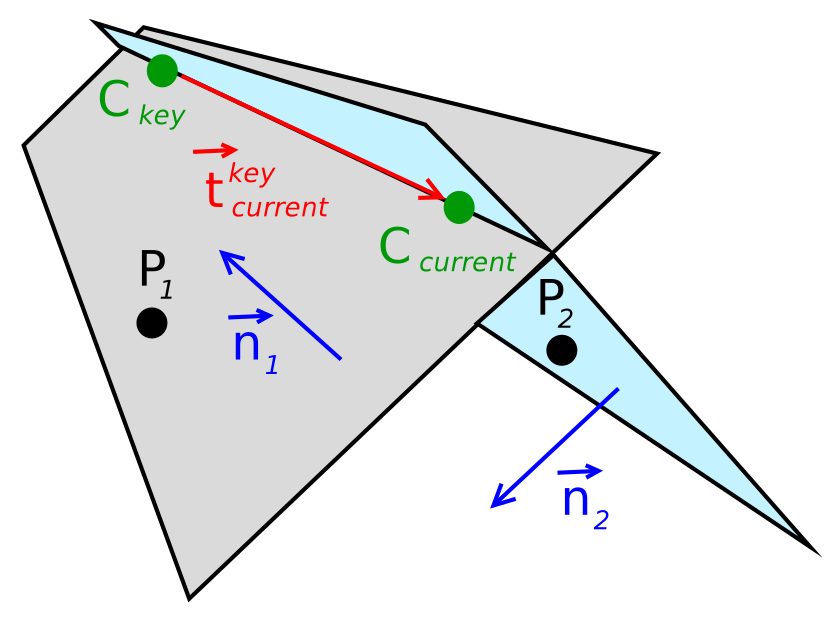
\includegraphics[width=0.7\textwidth]{TwoPoint}
	\caption[Intersección de planos epipolares]{Intersección de planos epipolares.}
	\label{imagen:epipolarPlanes}
\end{figure}


En la figura \ref{imagen:epipolarPlanes}, podemos observar que la intersección de estos planos tiene como lugar una recta cuya dirección es la del vector  $\overset { \rightarrow  }{ { \quad t }_{ key }^{ current } } $. Por tanto, es evidente que los vectores ${n}_{1}$ y ${n}_{1}$ son perpendiculares al vector $\overset { \rightarrow  }{ { \quad t }_{ key }^{ current } }  $ , y por tanto podemos calcular un vector con la misma dirección que este último como:


\begin{equation}
\overset { \rightarrow  }{ { t } } =\overset { \rightarrow  }{ { { n }_{ 1 } } } \times \overset { \rightarrow  }{ { { n }_{ 2 } } } 
\end{equation}

Por tanto se cumple:

\begin{equation}
 \overset { \rightarrow  }{ { t } } = s.\overset { \rightarrow  }{ {t }_{ key }^{ current } } 
\end{equation}

Donde s es un factor de escala.

Debido a esto, el vector de traslación unitario puede ser calculado como:

\begin{equation}
\overset { \rightarrow  }{ { t }_{ key}^{ current } } =\pm \quad \frac { \overset { \rightarrow  }{ t }  }{ \left\| \overset { \rightarrow  }{ t }  \right\|  } 
\end{equation}

Para determinar el signo, se  impone que la siguiente restricción:

\begin{equation}
(\overset { \rightarrow  }{ { f }_{ 1 } } \quad -\quad (\quad \overset { \rightarrow  }{ { { R }_{ 1 }^{ 2 } } } \quad .\quad \overset { \rightarrow  }{ { f }_{ 2 } } \quad ).\overset { \rightarrow  }{ { t }_{ current }^{ key } } >0
\end{equation}

La cual implica que los puntos característicos se encuentran al frente de la imagen.



\subsection{Selección de la función de error }

En general, es posible encontrar más de un par de parejas de correspondencias por imagen, por lo que es necesario estimar el vector de traslación unitario que reduzca el error grupal de correspondencias.

Una forma de hacer esto es realizar la triangulación de las correspondecias con el residual de rotación y  el vector unitario de traslación para un par de características del grupo, y calcular el error de reproyección para todas las correspondencias, y el vector de traslación que disminuya el error del grupo se considerará como la mejor estimación. Sin embargo, esto tiene un alto costo computacional debido a que en cada iteración deben ser nuevamente trianguladas los puntos característicos.

Debido a ello, y para conservar la simplicidad y reducir el costo computacional, se toma como función de error el producto punto entre el vector estimado y los vectores normales a los planos epipolares $\overset { \rightarrow  }{ { n }_{ i } } $ . En teoría, el producto punto entre el vector unitario de traslación y el normal al plano epipolar debe ser $0$, sin embargo debido a la resolución de la imagen, a la precisión de la detección de la característica, y a la profundidad del punto, esto no ocurre en general.

Una vez definida la función de error existen dos aproximaciones básicas para hallar la mejor estimación.
En presencia de un número significativo de correspondecias erróneas, se puede optar por métodos como RANSAC, para estimar el vector unitario de traslación que mejor se ajuste a un subconjunto del grupo de características, o en caso de tener una parte previa de filtrado de correspondencias, utilizar métodos iterativos como el de Gauss-Newton para hallar el vector de traslación que reduzca el error grupal.

En este trabajo se eligio emplear RANSAC debido a su simplicidad, costo computacional fijo, y robustez ante correspondencias erróneas.

\subsection{RANSAC}





\section{Extracción de residuales fotométricos}
\subsection{ Selección de parejas }

Actualmente la selección de parejas posee una esquema de  implementación basado en  CPU (figura 13) y  esquema similar basado en GPU (figura 14).\\

En ambos módulos se tienen las imágenes i e i+1, las cuales son la entrada del modulo de extracción de características.
En la salida de este módulo se tienen la ubicación de los puntos característicos en las imágenes y sus descriptores. Este módulo tiene a disposición 5 tipos de detectores en la versión en CPU y 2 tipos de detectores en la versión en GPU.\\

Posteriormente, el módulo de emparejamiento es el encargado de generar las parejas de correspondencias entre los puntos característicos de las dos imágenes, utilizando para ello algoritmos de emparejamiento como FLANN (del inglés: Fast Library for Approximate Nearest Neighbors)
y fuerza bruta. En la implementación en CPU se dispone de ambos algoritmos, mientras que la versión en GPU sólo implementa fuerza bruta.\\

Por último, el módulo de filtrado se encarga de seleccionar las mejores parejas entre las dos imágenes.  Este módulo es común en ambas versiones y se encuentra implementado en CPU.\\

\begin{figure}[H]
	\centering
	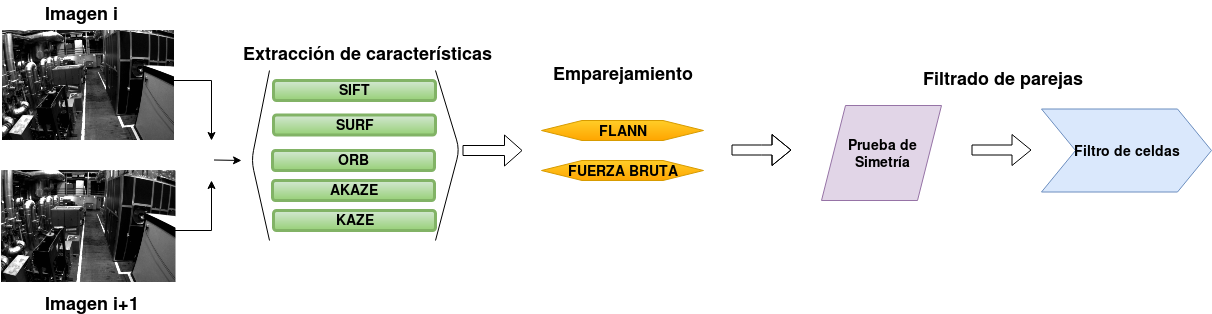
\includegraphics[scale=0.4]{Implementacion/DiagramaCPU2.png}
	\caption{Esquema general del módulo de extracción de parejas en CPU.}
	\label{fig:my_label}
\end{figure}


\begin{figure}[H]
	\centering
	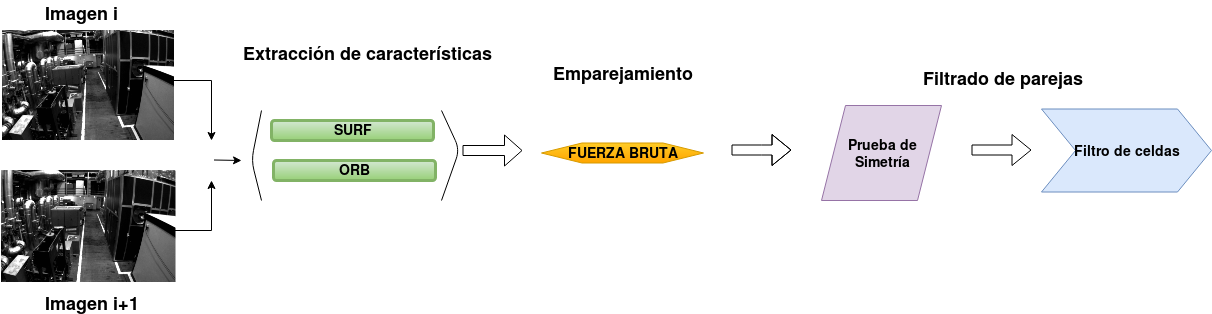
\includegraphics[scale=0.4]{Implementacion/DiagramaGPU2.png}
	\caption{Esquema general del módulo de extracción de parejas en GPU.}
	\label{fig:my_label}
\end{figure}

\subsubsection{Extracción de puntos característicos}

El modulo de extracción de puntos característicos en CPU dispone de detectores como SIFT, SURF, KAZE, AKAZE y ORB, mientras que la versión en GPU sólo posee SURF y ORB.\\

En la figura 15 se muestran la detección de puntos característicos  para una imagen perteneciente al EuRoC MAV Dataset \cite{0}. De izquierda a derecha se presenta la extracción de  puntos característicos para SIFT (1666 puntos), SURF (1504 puntos), KAZE (1865 puntos), AKAZE (1653 puntos) y ORB (1500 puntos) sobre la misma imagen. \\
\begin{figure}[H]
	
	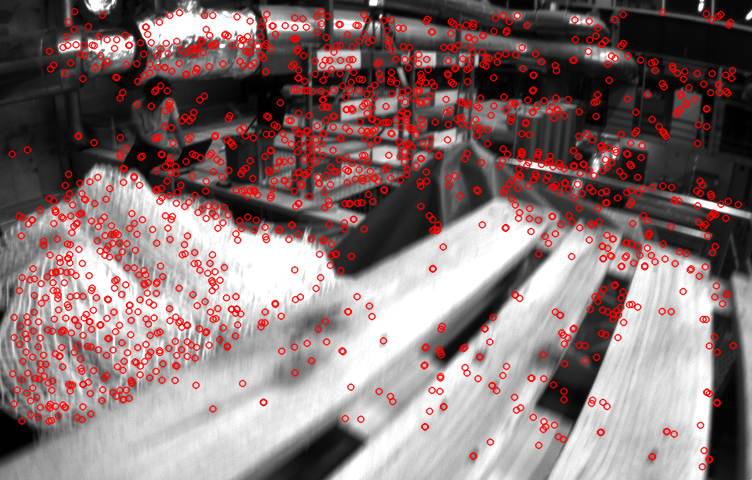
\includegraphics[scale=0.3]{Implementacion/DeteccionCaracteristicas/Imagen1SURF.png}
	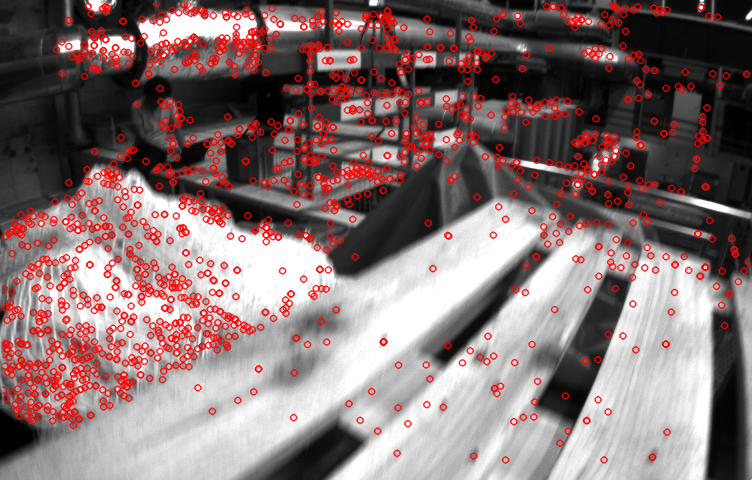
\includegraphics[scale=0.3]{Implementacion/DeteccionCaracteristicas/Imagen1SIFT.png}
	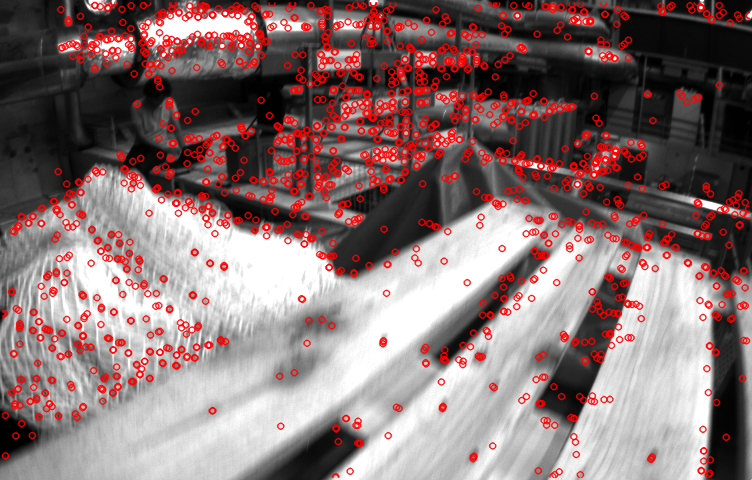
\includegraphics[scale=0.3]{Implementacion/DeteccionCaracteristicas/Imagen1KAZE.png}
	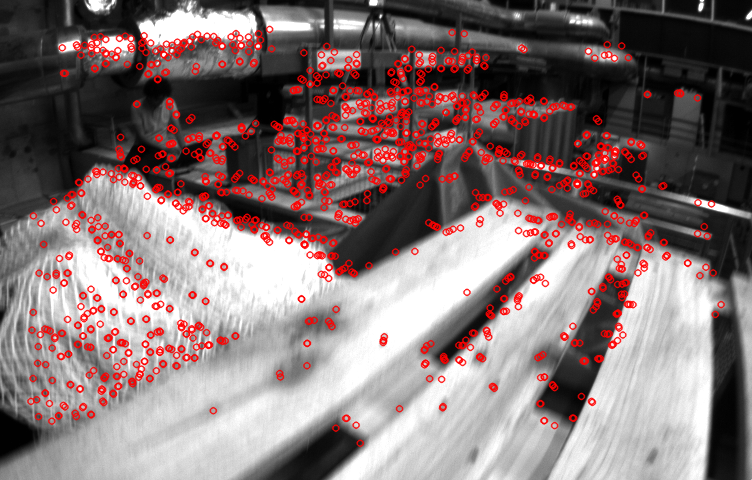
\includegraphics[scale=0.3]{Implementacion/DeteccionCaracteristicas/Imagen1AKAZE.png}
	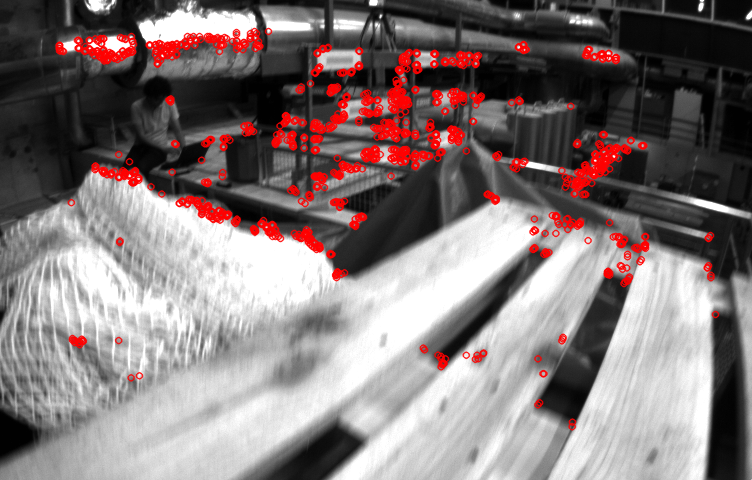
\includegraphics[scale=0.3]{Implementacion/DeteccionCaracteristicas/Imagen1ORB.png}
	\caption{Extracción de características.}
	\label{fig:my_label}
\end{figure}


\subsubsection{Filtrado de parejas}


Una vez se han identificado los puntos característicos en la imagen i y la i+1, se calculan los descriptores de las características detectadas y se procede a encontrar las correspondencias entre las dos imágenes. Para esta tarea se utiliza el método de vecinos más cercanos (KNN, del inglés:K Nearest Neighbors), el cual puede a su vez puede implementarse con algoritmos del tipo fuerza bruta o FLANN (del inglés: Fast Library for Approximate Nearest Neighbors). Este método se encarga de comparar el descriptor de un punto de referencia presente en la imagen i con los descriptores de los puntos de referencia de la imagen i+1 y determinar los k descriptores más cercanos al descriptor de la imagen i . En este caso la métrica de distancia puede corresponder a distancia euclidiana, en el caso de descriptores vectoriales, o a distancia Hamming, en el caso de descriptores binarios.\\

En esta implementación se utiliza k = 2, y se considera como una correspondencia aquellos casos donde la distancia entre el descriptor de la característica presente en la imagen i (D1) y su vecino más cercano en la imagen i+1 resulta 0.8 veces menor a la distancia entre D1 y el siguiente vecino de la imagen i+1. El valor de 0.8 se establece en correspondencia con el método de extracción de parejas de alta calidad establecido por David G. Lowe en \cite{1}.\\

Posteriormente se realiza una prueba de simetría entre parejas. En esta prueba, si el descriptor D1 de la característica  de la imagen i posee una correspondencia D2 en la imagen i+1, entonces al calcular la correspondencia desde D2 a la imagen i, debe resultar D1. Las parejas que no cumplan este criterio son descartadas.\\

En la figura 16 se presenta un ejemplo del filtrado  utilizando el detector SIFT. En la imagen i se detectaron 1666 puntos (figura 1) característicos, mientras que en la imagen i+1 se detectaron 1826. Luego de aplicar el filtrado de parejas por vecinos más cercanos y la prueba de simetría, la imagen i de la izquierda posee 882 correspondencias con la imagen i+1 presentada a la derecha.\\

\begin{figure}[H]
	
	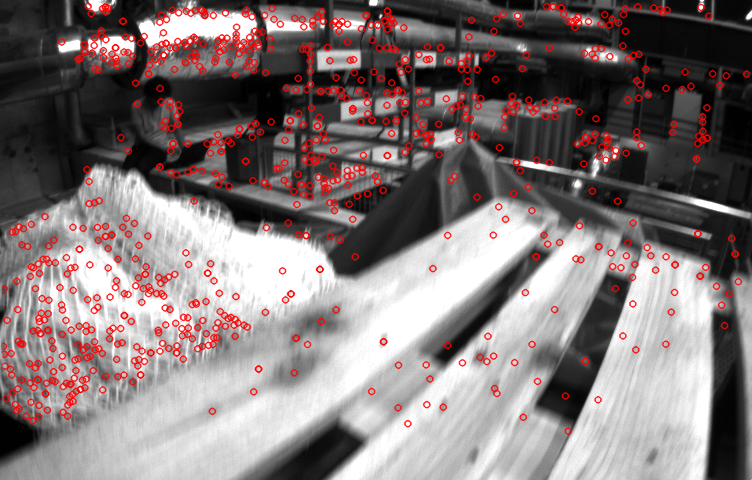
\includegraphics[scale=0.3]{Implementacion/FiltradoCorrespondencias/Imagen1.png}
	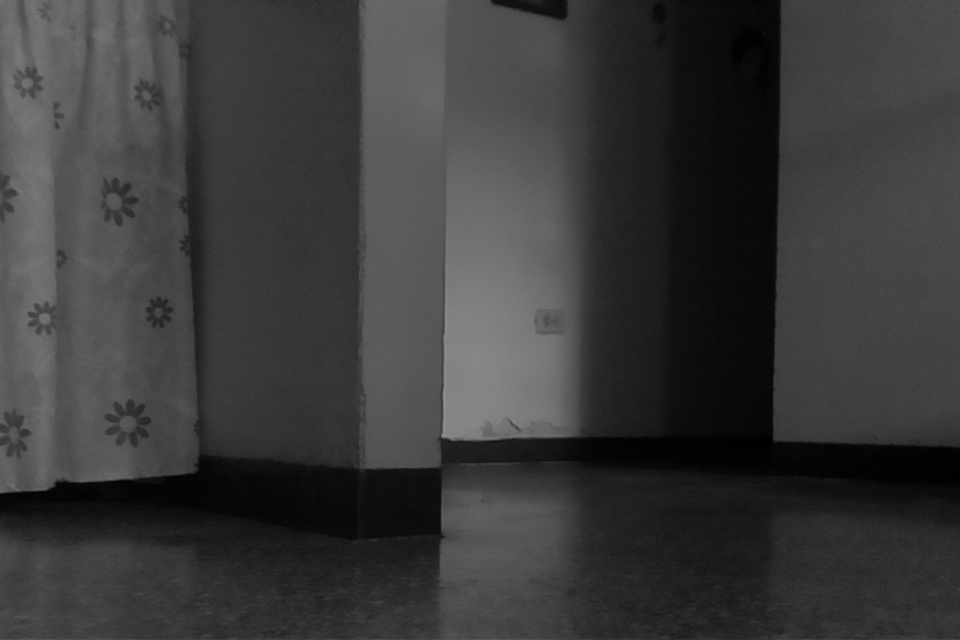
\includegraphics[scale=0.3]{Implementacion/FiltradoCorrespondencias/Imagen2.png}
	\caption{Salida del modulo de filtrado luego de la prueba de simetría.}
	\label{fig:my_label}
\end{figure}


Finalmente, se realiza una distribución espacial de las mejores parejas  sobre las imágenes i e i+1 utilizando un filtro de celdas. En este último,la imagen i es dividida en celdas de m x n pixeles. En esta implementación se m y n son el resultado de dividir el ancho y el largo de la imagen, respectivamente, por un mismo número entero k. \\

La figura 17 presenta dos imágenes en las que el filtro de celdas es aplicado. La imagen de la izquierda es el resultado de colocar las dimensiones de una imagen de resolución 752x480 píxeles, en celdas unitarias de aproximadamente 62x40 píxeles,
tomando k = 12,  generando por tanto 144 celdas y teniendo un total de 112 parejas finales luego de aplicado el filtrado. Por su parte, la imagen de la derecha es el resultado de fraccionar en 36 celdas la imagen original, tomando k = 6. En ésta, se tienen 34 parejas finales. \\


\begin{figure}[H]
	
	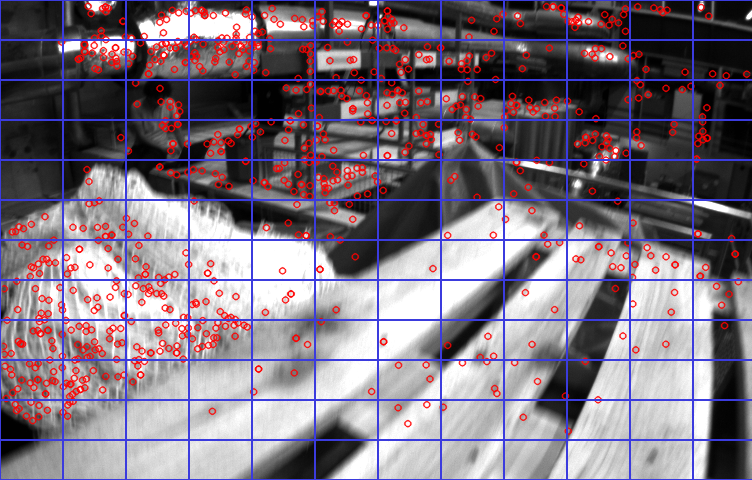
\includegraphics[scale=0.3]{Implementacion/FiltradoCorrespondencias/Imagen1Grid12.png}
	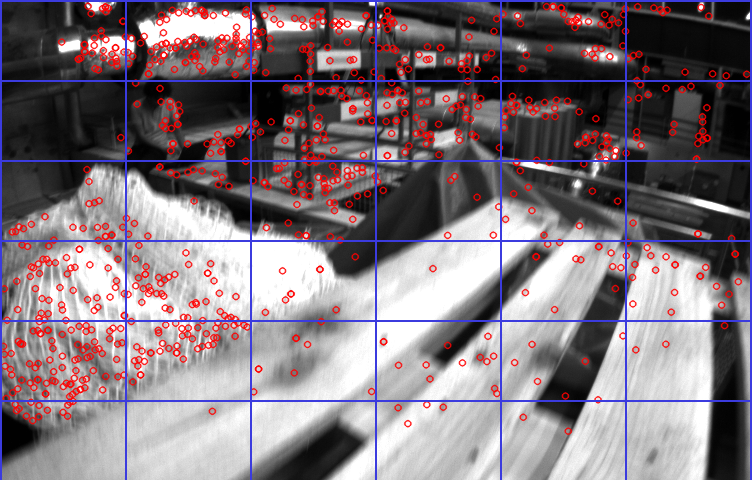
\includegraphics[scale=0.3]{Implementacion/FiltradoCorrespondencias/Imagen1Grid6.png}
	\caption{División de la imagen en celdas.}
	\label{fig:my_label}
\end{figure}


El criterio aplicado para seleccionar las mejores parejas y distribuirlas de forma homogénea sobre la imagen  consiste en seleccionar la mejor pareja  dentro de la región de la imagen correspondiente a la celda, y descartar a las demás parejas presentes. Se considera como mejor pareja a aquella que posea la menor distancia entre los descriptores de sus dos puntos característicos.\\

Las figuras 18 y 19 presentan el resultado final del modulo de filtrado de parejas con 36 y 144 celdas, respectivamente. Se puede observar que el filtro de celdas sólo es aplicado en los puntos característicos de la imagen i, ya que debido al movimiento del robot las puntos característicos se encuentran distribuidos de forma diferente en la imagen i+1 (imagen mostrada a la derecha) . \\

\begin{figure}[H]
	
	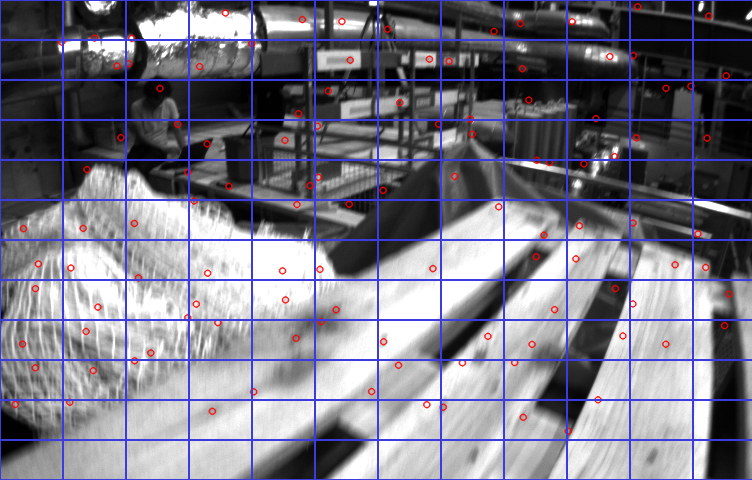
\includegraphics[scale=0.3]{Implementacion/FiltradoCorrespondencias/Imagen1BEST12.png}
	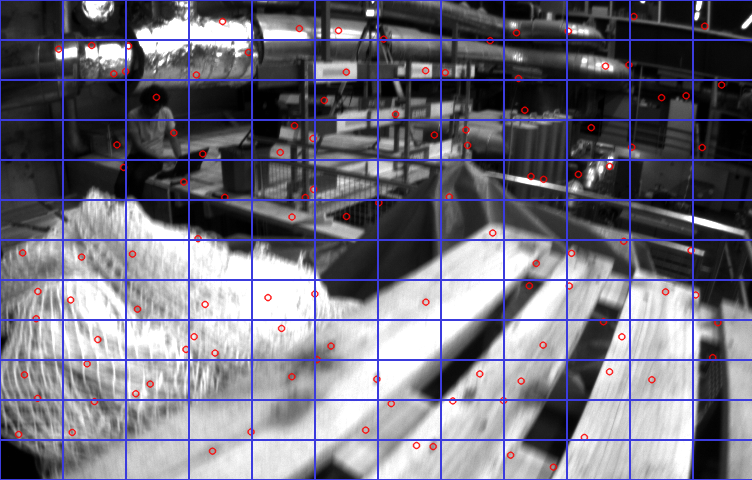
\includegraphics[scale=0.3]{Implementacion/FiltradoCorrespondencias/Imagen2BEST12.png}
	\caption{Filtrado de parejas con 144 celdas.}
	\label{fig:my_label}
\end{figure}


\begin{figure}[H]
	
	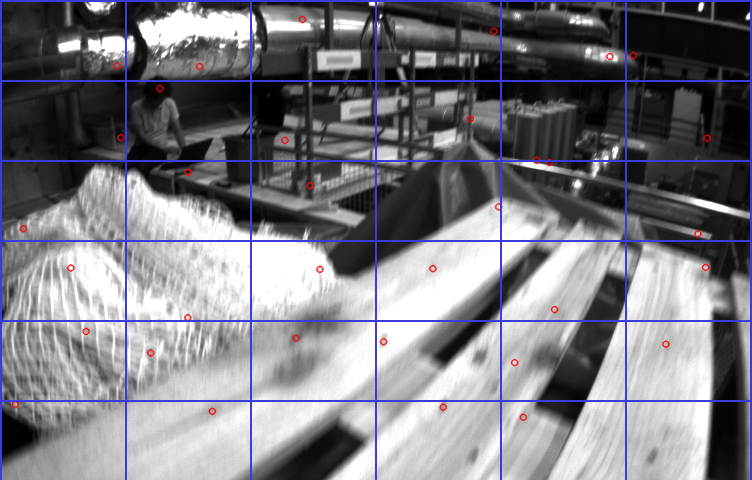
\includegraphics[scale=0.3]{Implementacion/FiltradoCorrespondencias/Imagen1BEST6.png}
	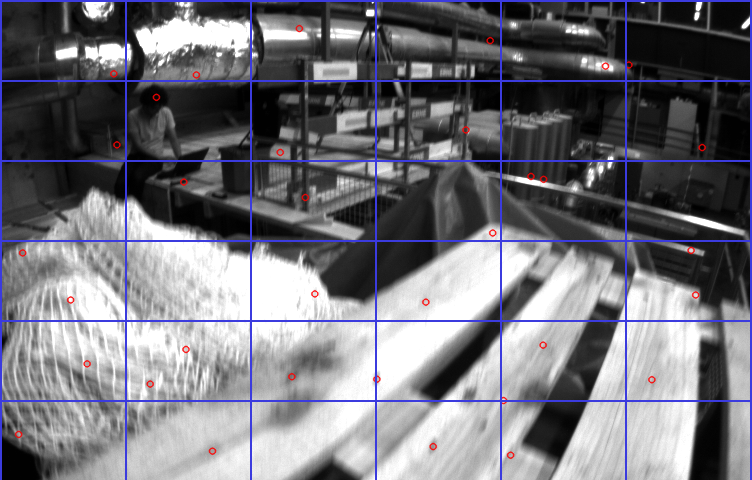
\includegraphics[scale=0.3]{Implementacion/FiltradoCorrespondencias/Imagen2BEST6.png}
	\caption{Filtrado de parejas con 36 celdas.}
	\label{fig:my_label}
\end{figure}

Cabe destacar que siempre que existan suficientes puntos característicos distribuidos en la imagen a la entrada de este módulo, el número de parejas finales será cercano al número de celdas. \\

Para evaluar el tiempo de cómputo del filtrado espacial se utilizó un equipo Intel ® Core 2 Duo CPU E8400 @ 3.00Ghz, dando como resultado un tiempo aproximado de 400 $\mu$s para 144, 121, 100, 81, 64, 49 y 36 celdas, teniendo como entrada 882 parejas.




%%%%%%%%%%%%%%%%%%%%%%%%%%%%%%%%%%%%%%%%%%%%%%%%%%%%%%%%%%%%%%%%%%%%%%%%%%%%%%%
\section{Resultados}


Hasta ahora se han presentado casos en los que se lidia con un par de imágenes. Por lo tanto se presenta un mosaico compuesto por tres imágenes del conjunto \textit{Espenky}, adicionalmente se tiene un error producido por el efecto paralaje. En este caso el algoritmo busca por la mejor linea de corte para cada par de imágenes por separado, pero logrando un mosaico final sin errores de discontinuidades.

En este ejemplo en particular se logra evidenciar una debilidad que tiene este algoritmo. A pesar de ser muy robusto al evadir objetos por la diferencia de texturas y bordes, es común que se cuente con discontinuidades visuales producto de cambios de iluminación.


\section{Resumen}

En esta sección se presentan los errores resultantes de las etapas de alineación, y que evitan que se logre un  mosaico que cumpla con el objetivo de aparentar ser una misma imagen. Luego del planteamiento del problema se exponen y describen distintos algoritmos que buscan una solución a estos.

En su mayoría estos algoritmos buscan reducir las discontinuidades entre imágenes producto de objetos en movimiento dentro de la escena, errores de alineación de objetos y texturas, y diferencias de iluminación. Al final del capítulo se presentaron los distintos resultados que muestran la efectividad de los algoritmos descritos, en primer lugar resultados concretos de los módulos por separado y finalmente con resultados de mosaicos completos de los conjunto de datos estudiados, aplicando para estos el sistema completo especificado al inicio del presente proyecto.

